
\section{Introduction to Dark Matter}
\pagenumbering{arabic}


Over the past three-four decades, mounting evidence has suggested that ordinary baryonic matter contributes only a small fraction of the total composition of the universe.  Gravitational lensing measurements,  x-ray observations, and galactic rotation curves lead to the conclusion that our galaxy is immersed in a dark matter halo which exceeds the mass of ordinary matter by an order of magnitude.  This theory, known as the Lambda Cold Dark Matter model, is supported by Planck's recent measurements of the Cosmic Microwave Background, which constrain the composition of the universe to be roughly 5\% baryonic matter, 27\% cold dark matter (CDM), and 68\% dark energy~\cite{Planck}.  While we know much about ordinary matter, we know very little about the larger components.  In particular, while we understand certain characteristics of the cold dark matter component, there is no consensus on its composition.   Before examining the experiments which seek to answer this question, we will first discuss what is currently known about nonbaryonic dark matter.

\subsection{Evidence for Dark Matter}

\subsubsection{Mass Measurements from Galactic Rotation Curves}

In the early 1930's Fritz Zwicky was the first to use the Virial theorem to determine the total mass of the Coma cluster of galaxies.  In his examination, Zwicky found that the velocities at large radii were too high to be consistent with the Newtonian prediction arising from the visible matter alone ~\cite{Zwicky}. This discrepancy was reinforced in the 1970's, when further data on the rotational velocity of spiral galaxies began to be collected.  Instead of the rotational velocity falling off as $\propto 1/\sqrt{r}$ beyond the radius of visible matter as one would expect, the rotational velocity rises for small radii, then asymptotes to a constant $ v \simeq 100-300 \; $~km/s for large radii in most galaxies~\cite{Persic,Battaner,Binney}.  The most widely accepted explanation of this phenomenon is that the disk galaxies are immersed in a dark matter (DM) halo such that $ M(r)/r $, where $M(r)$ is the total mass within a radius $r$, remains constant at large radii.  Such a halo could form from an isotropic sphere of an ideal gas at a uniform temperature.

\begin{center}
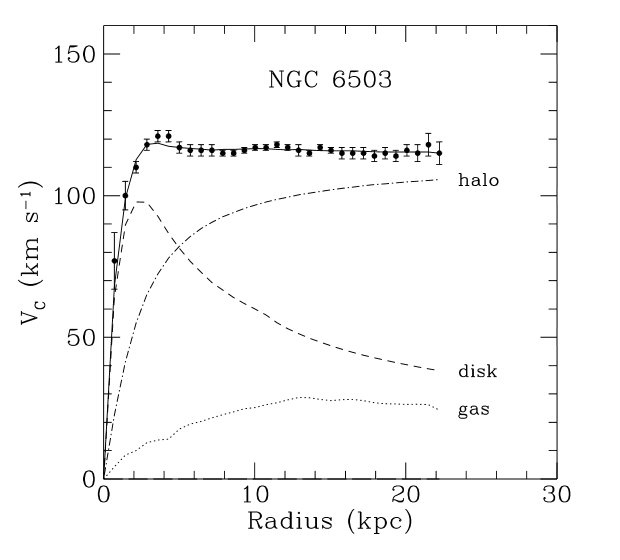
\includegraphics[scale=.7]{RotationCurve2.png}
\captionof{figure}{Rotation curve of galaxy NGC 6503.  The dotted line indicates the contribution of baryonic gas, the dashed line indicates the contribution of visible matter in the disk, and the dash-dotted line indicates the contribution of dark matter.  In the absence of dark matter the total velocity curve would fall off in a manner similar to the dashed line~\cite{Begeman}.}
\end{center}


Following Zwicky's footsteps, we can use the Virial theorem to calculate the luminous matter's contribution to the total mass of the Coma Cluster.  The theorem states that for a system of $N$ particles the time averaged total kinetic energy can be related to the time averaged total potential energy by
\begin{equation} \label{VirialTheorem}
\frac{1}{2} \sum_{i=1}^{N} \langle m_i v^2_i \rangle = -\frac{1}{2} \sum_{i=1}^N \langle \mathbf{r}_i \cdot {\mathbf{F}_i} \rangle
\end{equation} \label{VirialTheorem2}
where $m_i$,$v_i$, and $\mathbf{r}_i$ are the mass, velocity, and position of the $i$th particle with respect to the center of mass in a system of particles, and $\mathbf{F}_i$ is the force acting on the same particle.  Since the total force on a particle is the sum of all of the forces acting on it
\begin{equation}
\mathbf{F}_i = \sum_{j=1}^N \mathbf{F}_{ji}
\end{equation} \label{VirialTheorem3}
where $\mathbf{F}_{ji}$ is the force that particle $j$ applies on particle $i$.  Noting that a particle does not apply force to itself, and that Newton's third law of motion states that $\mathbf{F}_{ji} = -\mathbf{F}_{ij}$ we can rewrite the right hand side of the Virial theorem to be
\begin{equation} \label{VirialTheorem4}
 \sum_{i=1}^N \mathbf{F}_i \cdot \mathbf{r}_i = \sum_{i=1}^N \sum_{j<i} \mathbf{F}_{ji} \cdot \mathbf{r}_i +  \sum_{i=1}^N \sum_{j>i} \mathbf{F}_{ji} \cdot \mathbf{r}_i = \sum_{i=1}^N \sum_{j<i} \mathbf{F}_{ji} \cdot (\mathbf{r}_i - \mathbf{r}_j).
 \end{equation}
Using the law of gravitation to apply equation~\ref{VirialTheorem4} to a cluster of galaxies, the Virial theorem becomes
\begin{equation} \label{VirialTheorem5}
 \sum_{i=1}^{N} \langle m_i v^2_i \rangle = \sum_{i}^{N} \sum_{j<i} \left\langle  \frac{Gm_im_j}{r_{ij}} \right\rangle
 \end{equation}
where G is the gravitational constant.  The left hand side of this equation is the total mass, $M$, of the cluster of galaxies multiplied by the time and mass averaged squared velocity.  The right hand side is approximately equal to $\frac{GM^2}{R}$, where $R$ is the radius of the galaxy cluster.  Rearranging equation~\ref{VirialTheorem5}, we arrive at an equation which relates the total mass of the galaxy cluster to the mean square velocity
\begin{equation} \label{VirialTheorem6}
 M \approx \frac{ \langle v^2 \rangle R }{G}
\end{equation} 

The mean square velocity of a galaxy cluster can be estimated by calculating the one dimensional line of sight velocity via redshift.  Under the assumption of spherical symmetry
\begin{equation} \label{VirialTheorem7}
 \langle v^2 \rangle = 3 \langle (v_r - c \langle z \rangle)^2 \rangle
\end{equation} 
where $\langle z \rangle$ is the average redshift of the galaxy cluster, $v_r$ is the line of sight velocity, and c is the speed of light.  For the Coma cluster $\langle z \rangle = 0.0232$, which produces an estimate of $\langle v^2 \rangle \approx 6 \times 10^{12}$~m$^2$/s$^2$~\cite{ComaZ}.  Using the measured half-light radius of the Coma cluster ($R \approx 5 \times 10^{22}$ m) the total mass of the system in terms of solar mass ($M_{\odot}$) is found to be
\begin{equation} \label{VirialTheorem8}
M_{total} \approx 2 \times 10^{15} M_{\odot}.
\end{equation}

It is is also possible to measure the mass of a galaxy cluster from luminous matter alone.  The luminosity density of the universe around 445 nm has been observed to be 
\begin{equation}
j=1.0 \times 10^8 e^{\pm 0.26} h L_{\odot} \text{Mpc}^{-3},
\end{equation}
where $h=H_0/100$ is in the dimensionless units of 100 km/s/Mpc, $H_0$ is Hubble's constant, and $L_\odot$ is the luminosity of the Sun in the B band.  The critical mass density of the universe is given by
\begin{equation}
\rho_c = \frac{3H_0^2}{8 \pi G} = 1.88 \times 10^{-29} h^2 \text{g cm}^2,
\end{equation}
where $G$ is the gravitational constant.  The ratio of these two quantities defines the mass-to-light ratio, 
\begin{equation}
\Gamma = 2800 e^{\pm 0.3} h \frac{M_\odot}{L_\odot}
\end{equation}
which can be used to convert the luminosity of a galaxy cluster to an estimate of the mass contributed by luminous matter alone~\cite{Golwala}.

Comparing the mass calculated from the virial theorem to the mass measured from luminosity observations of the Coma cluster we see that the luminous components contribute only a small fraction of the total mass of the system~\cite{ComaZ}.
\begin{equation} \label{VirialTheorem9}
\frac{M_{lum}}{M_{total}} \approx \frac{2.3 \times 10^{14} M_{\odot}}{2 \times 10^{15} M_{\odot}} = 0.11
\end{equation}

\subsubsection{Mass Measurements from x-ray Gases}

Measuring the density profile of x-ray gases provides another technique to measure the total mass of a galaxy cluster.  The total mass of a dynamically relaxed galaxy cluster can be measured from the hydrostatic equilibrium equation, which can be derived from the Tolman-Oppenheimer-Volkoff equation for stellar structure by taking the nonrelativistic  limit of $c \rightarrow \infty$, such that 
\begin{equation} \label{HEq1}
\frac{dP}{dr} = -\frac{GM(r)}{r^2}\rho
\end{equation}
where $P$ is the pressure of the gas in a cluster, $G$ is the gravitational constant, $M(r)$ is the mass of the galaxy cluster within a particular radius, and $\rho$ is the density of the gas in the cluster~\cite{EinsteinGrav}.  From the ideal gas law we know that
\begin{equation} \label{HEq2}
P=\left(\frac{\rho}{\mu m_H}\right)kT
\end{equation}
where $\mu$ is the mean molecular weight ($\sim$0.6 as a fraction of the mass of a hydrogen atom for an ionized plasma~\cite{Belyanin}), $m_H$ is the mass of the hydrogen atom, and k is Boltzmann's constant.  Plugging this into equation~\ref{HEq1} yields
\begin{equation} \label{HEq3}
\frac{k}{\mu m_H}\left(T\frac{d\rho}{dr} + \rho\frac{dT}{dr} \right)=-\frac{GM(r)}{r^2}\rho
\end{equation}
Solving equation~\ref{HEq3} for $M(r)$ produces a measurement of the cluster's mass from x-ray gas density and temperatures
\begin{equation} \label{HEq4}
M(r) = -\frac{kT}{\mu m_H G}\left(\frac{d \; \text{ln}(\rho)}{d \; \text{ln}(r)} + \frac{d \; \text{ln}(T)}{d \; \text{ln}(r)}\right)r
\end{equation}
where the logarithms were introduced using the fact that 
\begin{equation}
\frac{r}{T}\frac{dT}{dr}=\frac{\frac{dT}{T}}{\frac{dr}{r}}=\frac{ d \; \text{ln}{T}}{d \; \text{ln}{r} }.
\end{equation} 
This mass measurement technique is complicated by the fact that the gas density and temperature of a galaxy cluster has spatial variation, as well as the fact that x-ray emission measurements are a two-dimensional projection of a three-dimensional object, which  produces complications when integrating x-ray spectra along lines of sight through the cluster. One method for simplifying the mass measurement, called the beta model, is to assume the cluster is made of isothermal, spherically symmetric gas.  In this case the density of the gas traces the density of the gravitational mass, such that
\begin{equation} \label{HBeta1}
\rho_{gas}(r) = \rho_0 \left(1 + \frac{r}{r_c}\right)^{-3\beta/2}
\end{equation}
where $r_c$ is the core radius, $\rho_0$ is the central density, and $\beta$ is a slope parameter~\cite{Vikhlinin}.  The core radius $r_c$ is defined using the intensity of x-ray observations such that $I(r_c)=\frac{1}{2}I(0)$, or more generally to be the radius at which $\frac{d^2 \; \text{ln}(I)}{d \; \text{ln}(r)^2}$ is maximized. In this model the mass measurement reduces to a derivation of the spatial density profile by determining the best fit parameters of $r_c$ and $\beta$ to the x-ray observations.  When this mass measurement technique is compared to mass measurements from luminous matter alone more evidence for dark matter arises. For example, using this technique the Virgo Cluster has been measured to have a total mass (within r $<$ 1.8Mpc) between $1.5 \times 10^{14} M_{\odot}$ and $5.5 \times10^{14} M_{\odot}$~\cite{Paradijs}. Comparing this to the mass measured from x-ray luminosity yields a ratio of
\begin{equation} \label{betamodelmass}
\frac{M_{lum}}{M_{total}} \approx \frac{4.75 \times 10^{13} M_{\odot}}{3.5 \times 10^{14} M_{\odot}} = 0.14.
\end{equation}

\subsubsection{Gravitational Lensing}


Gravitational lensing provides an independent method for measuring the mass of galaxy clusters and other astronomical objects.  Gravitational lensing can be divided into two categories -- strong lensing and weak lensing.  Strong lensing, in which a background light source is distorted into arcs around a massive foreground object, is a rare phenomenon which requires a light source and a very massive lens to be nearly in line with the observer.  When such a situation occurs the mass of the lens can be inferred from the angular width of the arc of light which is produced.  We turn to general relativity to derive the equation which produces this mass measurement.

The geodesic equation, which describes the path that a free particle travels, is given by
\begin{equation} \label{geodesic}
\frac{d}{d\tau} \left(g_{aj} \frac{dx^j}{d\tau} \right)-\frac{1}{2}\frac{\partial g_{ij}}{\partial x^a} \frac{dx^i}{d\tau}\frac{dx^j}{d\tau} = 0
\end{equation}
where $g_{\alpha j}$ is a metric, $\tau$ is the proper time, and $x^i$ is the four dimensional coordinate vector. For a spacetime in a vacuum outside of a spherically symmetric mass the appropriate metric to use is the Schwarzschild metric.  With units of $c=1$ it is given by
\begin{equation} \label{s-metric}
ds^2 = -\left(1-\frac{2GM}{r}\right)dt^2 + \left(1-\frac{2GM}{r}\right)^{-1}dr^2+r^2 d \theta^2 + r^2 sin^2 \theta d\phi^2.
\end{equation}
From the $t$ component of the geodesic equation we know that
\begin{equation} \label{geodesic-t}
\frac{d}{d \tau} \left(g_{tj}\frac{dx^j}{d\tau}\right) - \frac{1}{2} \frac{\partial g_{ij}}{\partial t} \frac{dx^i}{d\tau} \frac{dx^j}{d \tau} =0.
\end{equation}
The Schwarzschild metric does not depend on time, and is diagonal, therefore
\begin{equation} \label{geodesic-t-reduced}
\frac{d}{d \tau} \left(g_{tj}\frac{dx^j}{d\tau} \right) = \frac{d}{d \tau} \left(g_{tt}\frac{dt}{d\tau}\right) = -\frac{d}{d \tau}\left( \left(1-\frac{2GM}{r}\right)\frac{dt}{d\tau}\right) = 0.
\end{equation}
Equation~\ref{geodesic-t-reduced} is true if the quantity inside of the derivative is constant, leading us to the first constant of motion
\begin{equation}\label{first com}
E=\left(1-\frac{2GM}{r}\right)\frac{dt}{d\tau}.
\end{equation}
We now turn to the $\phi$ component of the geodesic equation
\begin{equation} \label{geodesic-phi}
\frac{d}{d \tau}\left(g_{\phi j}\frac{dx^j}{d\tau}\right) = \frac{d}{d \tau}\left(g_{\phi \phi}\frac{d\phi}{d\tau}\right) = -\frac{d}{d \tau}\left(r^2 sin^2 \theta \frac{d\phi}{d\tau}\right) = 0
\end{equation}
where we have once again used the fact that the metric does not depend on time and is diagonal to simplify the equation.  From this we arrive at the second constant of motion
\begin{equation} \label{second com}
l=r^2sin^2\theta \frac{d\phi}{d \tau}
\end{equation}
%If we assume motion in the equatorial plane then $\theta=\pi/2$, and the ratio 
%of the two constants of motion becomes
%\begin{equation} \label{com ratio}
%u \equiv \frac{l}{E} = \frac{r^2\frac{d\phi}{d\tau}}{(1-\frac{2GM}{r})\frac{dt}{d\tau}}=(1-\frac{2GM}{r})^{-1} r^2 \frac{d\phi}{dt}
%\end{equation}
%From this we get the equation of motion
%\begin{equation} \label{phi eqm}
%\frac{d\phi}{dt} = \frac{1}{r^2}(1-\frac{2GM}{r})u
%\end{equation}
Returning to the Schwarzschild metric, for a photon $ds^2$=0, and if we assume motion in the equatorial plane $\theta=\pi/2$ and $d \theta =0$, such that
\begin{equation} \label{photon metric}
-\left(1-\frac{2GM}{r} \right)dt^2 + \left(1-\frac{2GM}{r} \right)^{-1}dr^2+r^2 d\phi^2=0.
\end{equation}
From the two constants of motion we know that
\begin{equation} \label{dphi}
d\phi^2=\frac{l^2}{r^4 sin^4 \theta} d\tau^2
\end{equation}
and
\begin{equation} \label{dt}
dt^2=E^2\left(1-\frac{2GM}{r}\right)^{-2}d\tau^2
\end{equation}
Plugging equations~\ref{dphi} and~\ref{dt} into equation~\ref{photon metric} and simplifying yields
\begin{equation} \label{dr2}
dr^2= \left[E^2 - \left(1-\frac{2GM}{r}\right) \frac{l^2}{r^2}\right]d\tau^2
\end{equation} 
Finally, by dividing equation~\ref{dr2} by equation~\ref{dphi} we arrive at the equation of motion for light traveling in a Schwarzschild spacetime in polar coordinates
\begin{equation} \label{polar eqm}
\left(\frac{1}{r^2} \frac{dr}{d \phi} \right)^2 = \left(\frac{E}{l} \right)^2 - \left(1-\frac{2GM}{r}\right)\frac{1}{r^2} \equiv \left(\frac{1}{b}\right)^2 - \left(1-\frac{2GM}{r}\right)\frac{1}{r^2}
\end{equation}
The quantity $b \equiv l/E$ is known as the impact parameter, which represents the perpendicular distance between the center of attraction and the particle's initial trajectory.  To determine the change in the direction of light due to a gravitational field we must integrate $\frac{d\phi}{dr}dr $ from the minimum distance the light travels by the massive object, denoted as $R$, and then multiply by a factor of 2 to account for the symmetrical motion of the particle during its approach to the object. Note that at a distance $R$ the light is moving tangentially, such that $\frac{dr}{dt}=0$ and equation~\ref{polar eqm} becomes
\begin{equation} 
\frac{1}{b^2} = \left(1-\frac{2GM}{R}\right)\frac{1}{R^2}.
\end{equation} 
Therefore, we can rewrite equation~\ref{polar eqm} for any value of $r$ as
\begin{equation} \label{polar eqm-R}
\left(\frac{1}{r^2} \frac{dr}{d \phi}\right)^2 = \left(1-\frac{2GM}{R}\right)\frac{1}{R^2} - \left(1-\frac{2GM}{r}\right)\frac{1}{r^2}.
\end{equation}
Making the convenient substitution of $u \equiv R/r$, where $0 \leq u \leq 1$ in equation~\ref{polar eqm-R} yields 
\begin{equation} \label{polar eqm-u}
\left(\frac{du}{d\phi} \right)^2 = 1- u^2 - \frac{2GM}{r}(1-u^3).
\end{equation}
From this we can find an equation for the infinitesimal variation $d\phi$ in terms of $du$
\begin{equation} \label{dphi eqm}
d\phi = \frac{(1-u^2)^{-1/2}du}{\left[1 - \frac{2GM}{R}(1-u^3)(1-u^2)^{-1}\right]^{-1/2}}.
\end{equation}
A further substitution of $u \equiv \cos(\alpha)$, where $0 \leq \alpha \leq \pi/2$, leads (after some simplification) to the equation
\begin{equation} \label{final eqm}
d\phi = \left[1-\frac{2GM}{R}\left(\cos(\alpha) + \frac{1}{1+\cos(\alpha)}\right)\right]^{-1/2} d\alpha.
\end{equation}
\newpage
In most cases, the quantity $M/R<<1$, so we can use the approximation $(1+x)^n \approx 1+nx$ for small x in equation~\ref{final eqm} such that
\begin{equation}
d\phi = \left[1 + \frac{GM}{R} \left(\cos(\alpha) + \frac{1}{1+\cos(\alpha)}\right)\right]d\alpha.
\end{equation}
This is known as the "weak field" limit.  Integrating this expression from $0 \leq \alpha \leq \pi/2$ and multiplying by 2 to account for the two symmetrical legs of the light's trajectory provides an expression for the total azimuthal angle of the light.
\begin{equation} \label{polar angle}
\phi = 2 \int_{0}^{\pi/2} \left[1 + \frac{GM}{R} \left(\cos(\alpha) + \frac{1}{1+\cos(\alpha)}\right)\right] d\alpha = \pi + \frac{4GM}{R}.
\end{equation}
Noting that the first term, $\pi$, is the azimuthal angle of the light if no mass were present, we arrive at an equation that relates the angle of deflection of light to the total mass of the gravitational object. 
\begin{equation} \label{final GR}
\Delta \phi = \phi - \pi = \frac{4GM}{R} .
\end{equation}


In practice, we must go one step further to turn astronomical observations of gravitational lensing into a mass measurement.  Any observation of a lensed light source involves an observer viewing an image of the object after it passes by a gravitational lens.  This situation is depicted in Figure~\ref{fig:lensfigure}. To measure the mass of a lens we seek to relate the source position to the image position. Using the small angle approximation for $\theta$ and $\beta$ we can arrive at
\begin{equation} \label{lens eq 1}
D_S \theta = D_S\beta + D_{LS} \Delta \phi
\end{equation}
where $D_s=D_L+D_{LS}$ is the distance from the source plane to the observer.  Using equation~\ref{final GR}, and the fact that $R \approx \theta D_L$ this becomes
\begin{equation} \label{lens eq 2}
\theta = \beta + \frac{4GM D_{LS}}{\theta D_L D_S}.
\end{equation}
This is a quadratic equation with roots
\begin{equation} \label{lens roots}
\theta = \frac{ \beta \pm \sqrt{ \beta^2 + 4 \theta^2_E}}{2}
\end{equation}
where $\theta_E = \left(4GM \frac{D_{LS}}{D_S D_L} \right)^{1/2}$ is the angular size of the "Einstein ring" that forms when the source and lens are perfectly aligned.  If the quantities $D_{LS}$, $D_L$, and $\beta$ are known, equation~\ref{lens roots} can be used to measure the mass of the lens by measuring the angle of deflection $\theta$~\cite{Bin-Nun}. In the handful of cases in which this mass measurement has been carried out, it has been found to be consistent with dark matter models~\cite{Wu}. %Maybe put something like M_lum/M_tot < ?? here to be consistent with other sections


\begin{center} 
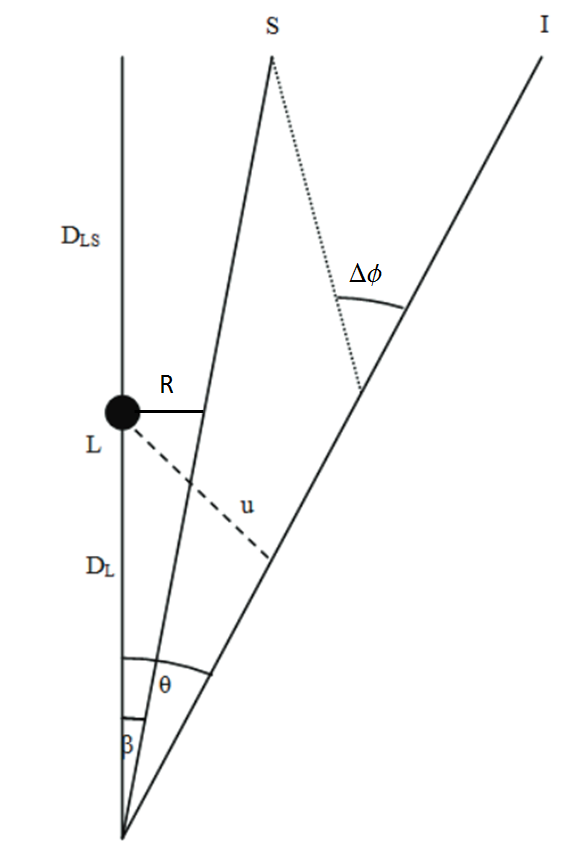
\includegraphics[scale=0.4]{LensEqFigure.png}
\captionof{figure}{A source emits light at position S.  The light is deflected by a massive lens at L, and causes the image seen by the observer to appear at an angle $\theta$.  D$_{LS}$, D$_L$, $\theta$, and $\beta$ are, respectively, the distance from the lens plane to the source plane, the distance from the lens plane to the observer, the angle of the image relative to the observer, and the angle of the source relative to the observer~\cite{Bin-Nun}. }
\label{fig:lensfigure}
\end{center}
 
Although there are only a few cases in which strong gravitational lensing can be observed, there are numerous cases of weak gravitational lensing.  Weak lensing occurs when the lensing mass isn't large enough for strong lensing, or if the source of light is not directly aligned with the lensing mass, resulting in a shear distortion of the image.  Measuring the mass of a weak lens is complicated by the fact that each light source has a unique, intrinsic ellipticity which typically dwarfs the magnitude of the image distortion.  This intrinsic ellipticity is known as ``shape noise'' in weak gravitational lensing studies.  In cases where many sources are lensed by the same object, the distortion from the lens can be measured by averaging over the many source images, taking advantage of their random intrinsic orientation.  In these cases, the measured shear distortion results from light being deflected by mass fluctuations along the line of sight.  In this case, the two dimensional lens equation (analogous to equation~\ref{lens eq 2}) in vector format is
\begin{equation} \label{2D lens}
\boldsymbol{\beta} = \boldsymbol{\theta} - \frac{D_{LS}}{D_S} \Delta \boldsymbol{\phi}(\boldsymbol{\xi})
\end{equation}
where $\boldsymbol{\xi}=D_{S}\boldsymbol{\theta}$ is the impact parameter.  The deflection angle can be calculated by integrating the 3D gravitational potential, $\boldsymbol{\Phi}(\mathbf{r})$, along the line of sight such that
\begin{equation} \label{3D angle}
\Delta \boldsymbol{\phi}(\boldsymbol{\xi}) = 2 \int \nabla_\perp \boldsymbol{\Phi}(\mathbf{r})dz = \nabla_\perp \left(2\int \boldsymbol{\Phi}(\mathbf{r}) dz \right) \equiv \nabla_\perp V.
\end{equation}
Assuming the angle between the image and the observer, $\boldsymbol{\theta}$, is small equation~\ref{2D lens} can be approximated with a first order Taylor series as
\begin{equation} \label{lens taylor}
\beta_{i}=A_{ij} \theta_{j}
\end{equation}
where $i$ corresponds to the $i^{th}$ component of the lens plane, $j$ corresponds to the $j^{th}$ component of the source plane, and 
\begin{equation} \label{dist matrix elements}
A_{ij}=\frac{ \partial \beta_i}{\partial \theta_j} = \delta_{ij} - \frac{ \partial \Delta \phi_i( \boldsymbol{\theta}) }{\partial \theta_j} = \delta_{ij} - 
\frac{ \partial ^2 V(\boldsymbol{\theta})} {\partial \theta_i \partial \theta_j}
\end{equation}
are the elements of a Jacobian distortion matrix, $\mathbf{A}$, which describes the isotropic dilation and anisotropic distortion due to convergence and shear effects.  The distortion matrix can be written in terms of the convergence, $\kappa$, which increases the size of the image while conserving brightness, and the shear, $\gamma$, which distorts the image tangentially around the lens.  
\begin{equation} \label{dist mat}
A_{ij}=(1-\kappa) \left(\begin{matrix} 1 & 0 \\ 0 & 1 \end{matrix} \right) - \gamma \left(\begin{matrix} \cos(2\phi) & \sin(2\phi) \\ \sin(2\phi) & -\cos(2\phi) \end{matrix} \right) 
\end{equation}
Equations~\ref{dist matrix elements} and~\ref{dist mat} offer a relationship between the observable quantities $\kappa$ and $\gamma$, and the gravitational potential $V$.
\begin{equation} \label{gamma1}
\gamma_1 \equiv \gamma cos 2\phi= \frac{1}{2} \left[\frac{ \partial ^2 V(\boldsymbol{\theta})}{\partial \theta_1^2} - \frac{ \partial^2 V(\boldsymbol{\theta})}{\partial \theta_2^2} \right]
\end{equation}
\begin{equation} \label{gamma2}
\gamma_2 \equiv \gamma \sin (2\phi) = \frac{ \partial^2 V(\boldsymbol{\theta})}{\partial \theta_1 \partial \theta_2}
\end{equation}
\begin{equation} \label{kappa}
\kappa = \frac{1}{2} \nabla^2 V(\boldsymbol{\theta})
\end{equation}
where equation~\ref{gamma1} comes from $A_{11}-A_{22}$, equation~\ref{gamma2} comes from $A_{12}-A_{21}$, and equation~\ref{kappa} comes from $tr(A)$.  Since $\kappa$ is equal to half the Laplacian of the projected gravitational potential, $V$, it is directly proportional to the mass density of the lens.  The shear component $\gamma_1$ corresponds to elongation and compression along the $x$ and $y$ directions, and the component $\gamma_2$ describes elongation and compression along the diagonal $x=y$ and $x=-y$ directions.  In the case of weak lensing, the mass measurement then reduces to a measurement of the shear and convergence produced by the lens~\cite{Pires}. As with strong gravitational lensing, weak gravitational lensing mass measurements have been found to be consistent with dark matter models~\cite{Wu}.


\begin{center} \label{lensfigure}
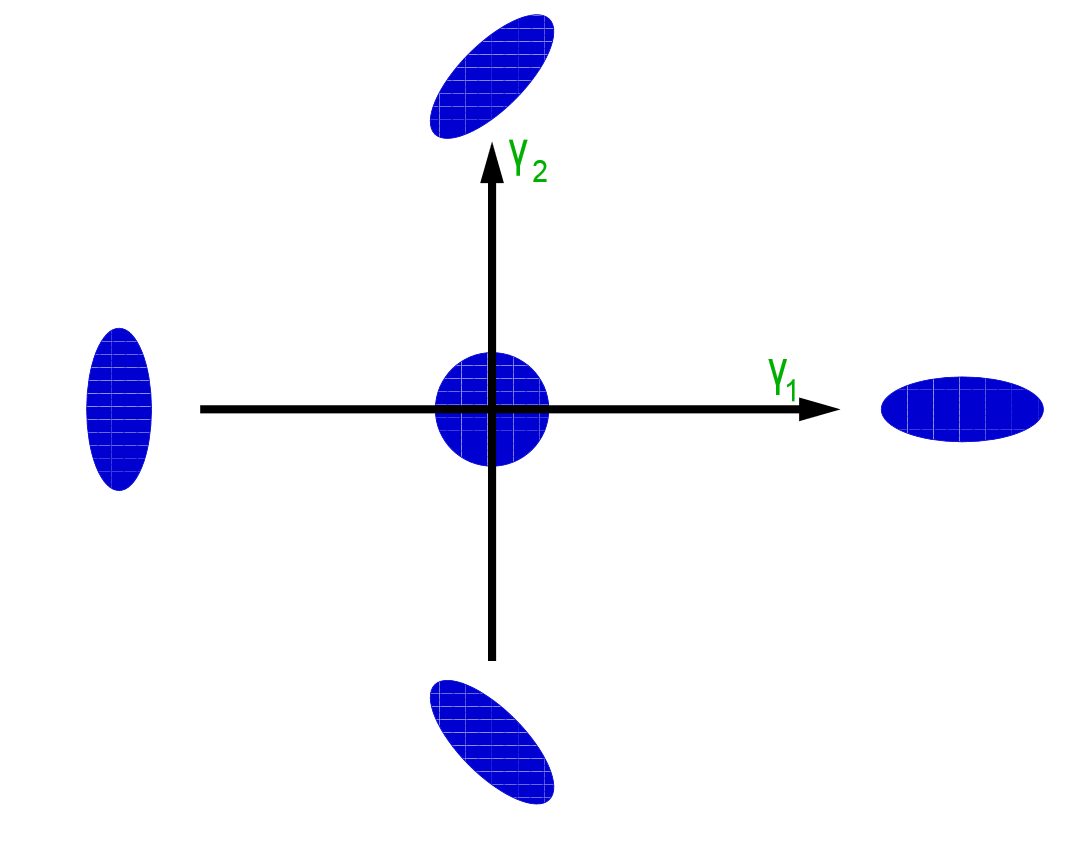
\includegraphics[scale=0.3]{GammaOneGammaTwo.png}
\captionof{figure}{An illustration of how positive and negative $\gamma_1$ and $\gamma_2$ distort an object with initial ellipticity of zero~\cite{Refregier}. }
\end{center}

%trace of A equation
%\begin{equation}
%tr(\mathbf{A})=2-\frac{\partial^2V(\boldsymbol{\theta})}{\partial\theta^2_1} - \frac{\partial^2 V(\boldsymbol{\theta})}{\partial \theta^2_2} = 2-\nabla^2V(\boldsymbol{\theta})=2(1-\kappa)
%\end{equation}
 
One of the most famous instances of weak lensing evidence for dark matter is a collision of two galaxies clusters known as the Bullet Cluster.  The baryonic matter in each galaxy cluster is predominantly in the form of hot gas.  Electromagnetic interaction causes the gas to to slow down and concentrate in the center of the collision.  In the absence of dark matter, gravitational lensing measurements should be correlated with the hot gas, since it is the dominant luminous mass in the system.  However, if dark matter was a dominant mass component in the Bullet Cluster it would not be slowed by electromagnetic interactions and would pass through the collision without significant perturbation. Indeed, weak gravitational lensing observations show that the majority of the mass in the Bullet Cluster passed through the collision rather than concentrating at the center like the luminous matter, suggesting that dark matter is present in abundance over the baryonic matter of the two galaxy clusters~\cite{Clowe}.


\begin{center} \label{bulletcluster}
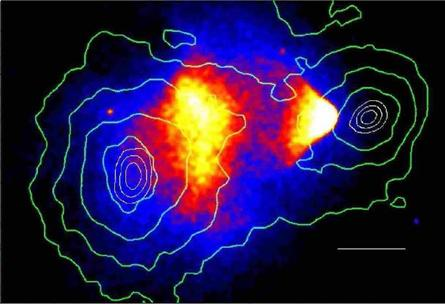
\includegraphics[scale=1]{bulletcluster.jpg}
\captionof{figure}{X-ray image of the baryonic mass in the Bullet cluster, overlayed with mass contours derived from weak lensing measurements.  The one, two, and three sigma confidence intervals for the center of the mass distributions are indicated by the white countours, and the white bar indicates a distance of 200 kpc.  The separation of the dominant mass component from the baryonic matter indicates the presence of dark matter~\cite{Clowe}. }
\end{center}
 

\subsubsection{Cosmological Evidence}

The early universe was filled with a hot, dense plasma of electrons and baryons.  At this time photons scattered off of the free electrons, restricting their movement across the universe.  As the universe cooled below the binding energy of hydrogen (13.6 eV) protons and electrons began to combine, forming neutral hydrogen atoms.  At this point, approximately 400,000 years after the big bang,  photons and electrons decoupled and the photons began traveling with a mean free path the size of the universe.  These photons produced the Cosmic Microwave Background (CMB) that we see today (Figure~\ref{fig:CMB_Planck}).  The radiation is extremely isotropic and exhibits a black-body spectrum at a red shifted temperature of 2.72 K.  The frequency spectrum, temperature fluctuations, and polarization of the CMB all contain a vast amount of information about the formation of the universe.  Here, we focus on just one of these properties. 



\begin{center} 
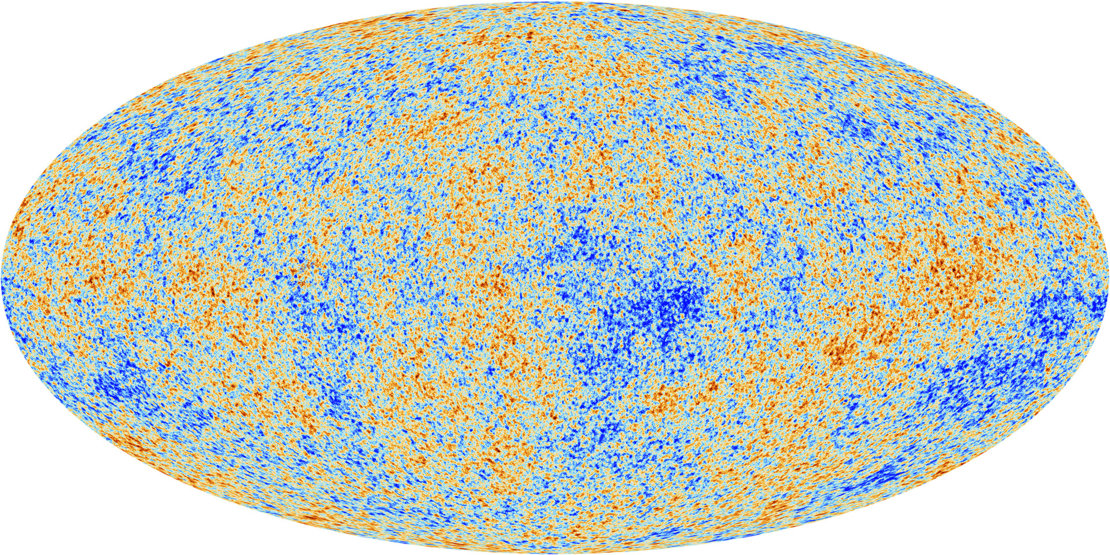
\includegraphics[scale=0.3]{CMB_Planck.jpg}
\captionof{figure}{The latest measurement of the CMB temperature anistropies from Planck data~\cite{Planck}, after contrast enhancement, and removing the dipole moment caused by the movement of the milky way.}
\label{fig:CMB_Planck}
\end{center} 

In 1991 the COBE satellite observed small (1 part in 10,000) fluctuations in the average temperature of the CMB~\cite{smoot1991first}.   Since then, the result has been confirmed by numerous ground based telescopes, as well as the WMAP and Planck satellites~\cite{Planck}.  We see these temperature fluctuations projected on a 2D spherical surface, so it is typical to expand them in terms of spherical harmonics defined by
\begin{equation}\label{Ylm}
Y_{lm}=\sqrt{\frac{2l+1}{4\pi} \frac{(l-m)!}{(l+m)!}}P_l^m(\cos\theta)e^{im\phi}
\end{equation}
where $l=0,...,\infty$, $-l \le m \le l$, and $P_l^m$ are associated Legendre polynomials.  The temperature fluctuations can then be written as
\begin{equation}\label{dTdT0}
f(\theta,\phi) \equiv \frac{\delta T(\theta,\phi)}{T_0} = \sum_{l=0}^{l=\infty} \sum_{m=-l}^{m=l} a_{lm} Y_{lm}(\theta,\phi)
\end{equation}
where $T_0$ is the average temperature of the CMB and $a_{lm}$ are the coefficients of expansion. Since the spherical harmonics are orthonormal
\begin{equation}\label{alm}
a_{lm} = \int_{\theta=-\pi}^{\pi}\int_{\phi=0}^{2\pi} f(\theta,\phi)Y_{lm}^*(\theta,\phi) d\Omega.
\end{equation}
The $a_{lm}$ coefficients represent a deviation from the average temperature  $T_0$, so their ensemble average is zero
\begin{equation}
\mean{a_{lm}} = 0
\end{equation}
and their variance, $\mean{|a_{lm}|^2}$, gives a measure of the typical size of $a_{lm}$.  The temperature fluctuations are isotropic and therefore independent of m, so
\begin{equation}\label{alm_var2}
\mean{|a_{lm}|^2}=\frac{1}{2l+1} \sum_{m}\mean{|a_{lm}^2|} \equiv C_l
\end{equation}
where the function $C_l$ is referred to as the angular power spectrum of the temperature fluctuations.  The angular power spectrum is related to contribution of the multipole $l$ to the temperature variance by
\begin{align}\label{powerspec}
\mean{\left(\frac{\delta T(\theta,\phi)}{T_0} \right)^2} \begin{aligned} = \end{aligned} \mean{\sum_{lm}a_{lm}Y_{lm}(\theta,\phi)\sum_{l'm'}a_{l'm'}^*Y_{l'm'}^*(\theta,\phi)} \nonumber \\
\begin{aligned} = \end{aligned} \sum_{ll'}\sum_{mm'}Y_{lm}(\theta,\phi)Y_{l'm'}^*(\theta,\phi)\mean{a_{lm}a_{l'm'}^* } \\
\begin{aligned} = \end{aligned} \sum_l C_l \sum_m |Y_{lm}(\theta,\phi)|^2 = \sum_l \frac{2l+1}{4\pi}C_l  \nonumber
\end{align}
where we have used the the closure relation
\begin{equation}\label{closure}
\sum_m |Y_{lm}(\theta,\phi)|^2 = \frac{2l+1}{4\pi}
\end{equation} and the fact that
\begin{equation}\label{alm_var1}
\mean{a_{lm}a_{l'm'}^*} = \delta_{ll'}\delta{mm'}\mean{|a_{lm}|^2}
\end{equation}
since the $a_{lm}$ coefficients are independent random variables~\cite{Kurki-Suonio}.


Cosmological models predict the variance of the $a_{lm}$ expansion coefficients, and therefore predict the angular power spectrum and the contribution of each multipole to the temperature variance.  By measuring the angular power spectrum of the CMB and comparing to the $C_l$ values predicted by each model we can learn about the composition of the universe.  The temperature fluctuations of the CMB are typically plotted in terms of $D_l \equiv l(l+1)C_l/(2\pi)$ with units of $\mu$K$^2$ versus the multipoles $l$ as shown in Figure~\ref{fig:PS_Planck}.

\begin{center} 
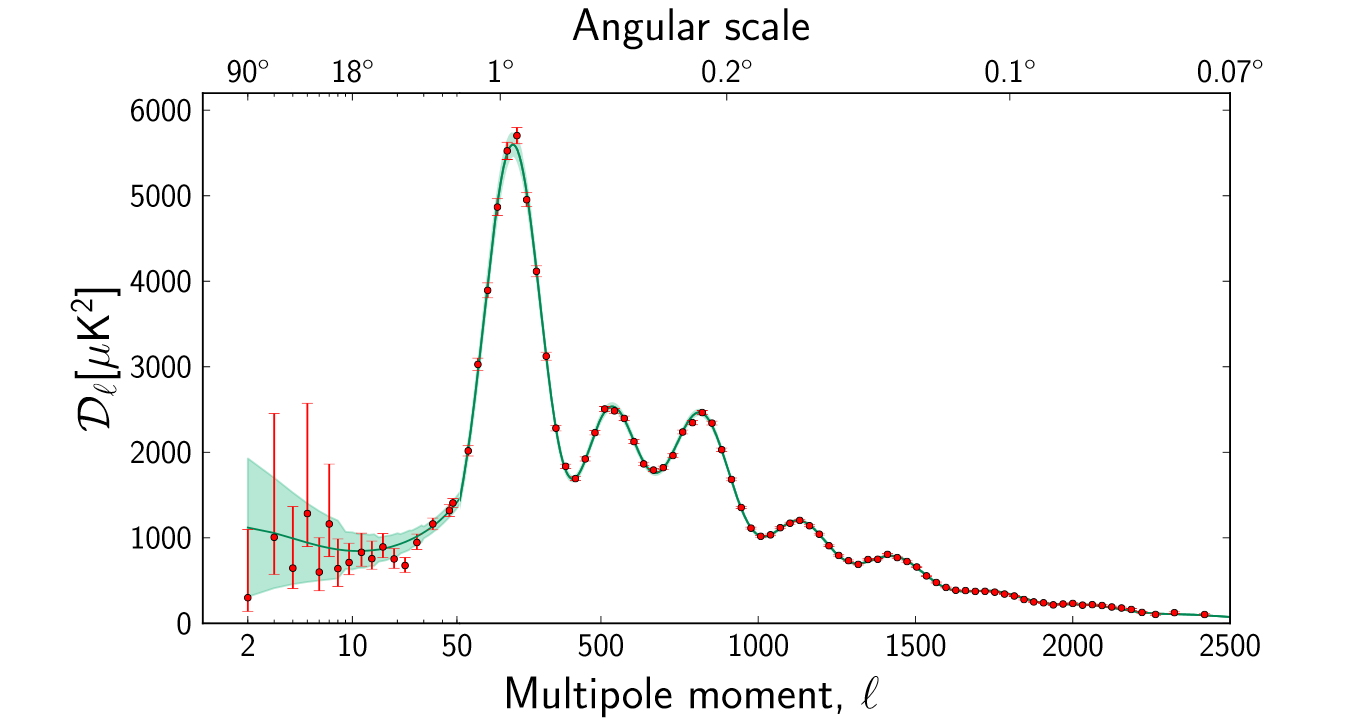
\includegraphics[scale=0.4]{PS_Planck.png}
\captionof{figure}{The power spectrum of temperature fluctuations from the CMB based on data from Planck~\cite{Planck}. The error bars at high multipole moments are smaller than the size of the data points.}
\label{fig:PS_Planck}
\end{center} 


To understand the wealth of information present in Figure~\ref{fig:PS_Planck} we must first understand the origin of the temperature fluctuations in the early universe.  Prior to recombination the primordial plasma consisted of anisotropic regions of varying density. Over-dense regions of matter would gravitationally attract more matter.  As this happened, heat from photons scattering off of free electrons would produce an increase in pressure, counteracting the force of gravity and pushing baryonic matter away from the high density regions.  As these two processes competed they produced oscillations in the distribution of baryonic matter, which we refer to as Baryon acoustic oscillations (BAO).  After recombination, the photons diffused through the baryonic matter, removing the source of pressure, ending the oscillating process, and leaving a shell of over-dense baryonic matter at the origin of the anisotropy and at a fixed radius called the sound horizon.

The first peak in Figure~\ref{fig:PS_Planck} details the curvature of the universe. If the universe had positive curvature the light from the CMB would be magnified, shifting the first peak to lower multipole in Figure~\ref{fig:PS_Planck}.  Likewise, in a negatively curved universe the scale of the temperature fluctuations in the CMB would appear diminished, shifting the first peak to higher multipole.  The observed location of the first peak, close to $l\sim$200, turns out to be consistent with a flat universe.  

The second peak in Figure~\ref{fig:PS_Planck} details the amount of baryonic matter in the universe.  Baryons add mass to the system during the oscillating process described above.  This additional inertia forces the primordial plasma to travel farther before recoiling back to the center of the anisotropy, much like adding a mass to the end of a spring.  The odd numbered peaks in Figure~\ref{fig:PS_Planck} are associated with how far the plasma compresses during BAO and are enhanced by the presence of additional baryons, as shown in Figure~\ref{BAO}.  The even numbered peaks are associated with how far the plasma rebounds during BAO and are unaffected by the presence of additional baryons.  Therefore, the presence of baryons enhances the size of the odd peaks over the even peaks such that a smaller second peak in Figure~\ref{fig:PS_Planck} corresponds to a larger amount of baryonic matter in the universe.  The latest results from Planck indicate that baryonic matter makes up $4.82 \pm 0.05\%$ of the universe~\cite{Planck}.


\begin{center} 
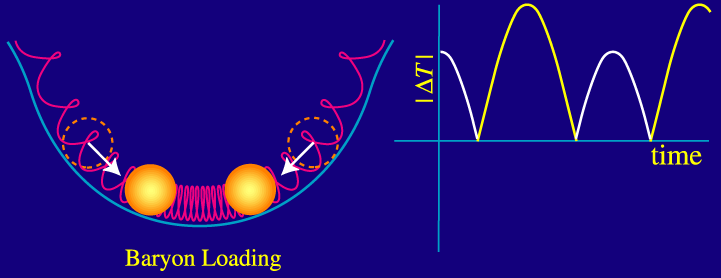
\includegraphics[scale=0.7]{BAO.png}
\captionof{figure}{A depiction of the effect of baryons on the oscillating plasma during BAO.  The mass of the baryons loads down the plasma, producing an asymmetry in the oscillations in which the plasma compresses further toward the minimum of the potential well. Since the CMB power spectrum does not care about the sign of the fluctuation, we see that the odd numbered peaks become enhanced over the even numbered peaks~\cite{Whu}. }
\label{BAO}
\end{center} 

The third peak in Figure~\ref{fig:PS_Planck} details the amount of dark matter in the universe.  Since the very early universe was dominated by photon-baryon interactions, the outward pressure caused the gravitational potential of the BAO system to decay in such a way that it drove the amplitude of oscillations higher.  With higher dark matter density this driving effect is diminished (since dark matter does not rebound) and the overall magnitude of the peaks becomes smaller.  Although this effects all of the peaks in Figure~\ref{fig:PS_Planck} it is only distinguishable in the third peak.  Furthermore, as with ordinary matter, dark matter was gravitationally attracted to areas with higher density.  Since dark matter does not interact through the electromagnetic force it was unaffected by the increasing photon pressure which produced acoustic oscillations in baryons.  As a result, a higher density of dark matter corresponded to a larger gravitational potential well for baryons to fall into during their oscillations, increasing the amplification of BAO on the odd numbered peaks.  Therefore, the height of the third peak tells us the amount of dark matter that is present in the universe~\cite{Whu}. The Planck observations indicates that dark matter makes up $25.8 \pm 0.4\%$ of the universe.  The remaining $69.4 \pm 1.0\%$ of the universe is made up of dark energy~\cite{Planck}.


\subsection{Dark Matter Candidates}

\subsubsection{The $\Lambda$CDM Model}
To further examine the properties of dark matter it is useful to introduce a quantitative measure for the composition of the universe.  Friedmann's equation, which describes the expansion of space in a homogeneous and isotropic universe, is given by
\begin{equation}\label{Friedmann's}
\frac{\dot{a}^2 + kc^2}{a^2} = \frac{8 \pi G \rho + \Lambda c^2}{3}
\end{equation}
where $a$ is the scale factor of the universe, $k$ is the spatial curvature of the universe (equivalent to one sixth of the Ricci Scalar), $c$ is the speed of light, $G$ is the gravitational constant, $\rho$ is the density of the universe, and $\Lambda$ is the cosmological constant. Einstein's field equations,
\begin{equation}\label{EFQ}
G_{\mu\nu} = \frac{8 \pi G}{c^4} T_{\mu\nu}
\end{equation}
provide an expression for the cosmological constant, $\Lambda$.  We can split the stress energy tensor into two terms, one describing matter and the other describing the vacuum, such that $T_{\mu\nu}=T_{\mu\nu}^{matter}+T_{\mu\nu}^{vac}$.  Since the stress energy tensor is given by
\begin{equation}\label{StressTensor}
T_{\mu\nu} = (\rho + p)U_{\mu}U_{\nu} + pg_{\mu\nu}
\end{equation}
and to maintain Lorentz invariance $p^{vac} = -\rho^{vac}$, we can write the vacuum component of the stress energy tensor as
\begin{equation}\label{StressTensorVac}
T_{\mu\nu}^{vac}=-\rho^{vac} g_{\mu\nu}.
\end{equation}
If we identify the vacuum energy density as
\begin{equation} \label{VacEnergyDens}
\rho^{vac}=\frac{\Lambda c^2}{8\pi G}
\end{equation}
then Einstein's field equation takes on the familiar form
\begin{equation}\label{EFQ2}
G_{\mu\nu} + g_{\mu\nu}\Lambda= \frac{8 \pi G}{c^4} T_{\mu\nu}^{matter}
\end{equation}
where $G_{\mu\nu}$ is the Einstein tensor, $g_{\mu\nu}$ is the metric tensor, $G$ is the gravitational constant, and $\Lambda$ is the cosmological constant.
Setting the normalized spatial curvature $k = 0$ in Friedmann's equation(representing a flat universe), one can find the critical density for which the universe is spatially flat to be
\begin{equation}\label{RhoC}
\rho_c = \frac{3}{8 \pi G}\frac{\dot{a}^2}{a^2}
\end{equation}
where $\rho_c = \rho^{vac}+\rho$.
Recognizing Hubble's constant to be $ H_0 = \frac { \dot{a}}{a} $, we can rewrite this as
\begin{equation}\label{RhoC2}
\rho_c =\frac{3H_0^2}{8 \pi G}
\end{equation}
where $H_0$ is the present value of the Hubble constant~\cite{Javorsek}. The current experimental value for $H_0$ in the dimensionless units 100 km/s/Mpc is $ h \sim 0.7 $ with an uncertainty of $\sim5\%$~\cite{Littleh}.  We can then define the density parameter as 
\begin{equation} \label{Omega}
\Omega=\frac{\rho}{\rho_c}=\frac{8 \pi G \rho}{3 H_0^2}.
\end{equation}
If $\Omega$ is larger than unity the universe is spatially closed, and if $\Omega$ is less than unity the universe is spatially open. This density parameter can be split into components, such that for a particular component $x$
\begin{equation} \label{OmegaComp}
\Omega_x = \frac{\rho_x}{\rho_c}.
\end{equation}

Detailed cosmological studies have concluded that all the luminous matter in the universe has a density parameter of $\Omega_{lum} \lesssim 0.01$.  This information, combined  with the fact that analysis of galactic rotational velocities implies $> $90\% of the mass in galaxies is dark leads to the conclusion that $\Omega_{DM} \geq 0.09$.  This is only a lower limit on the dark matter density parameter, since most rotation curves remain flat out to the largest radii at which they can be measured and it can be assumed that the DM halos extend even farther out.


It is possible that baryonic DM alone could be responsible for the dark matter halos.  However, other analyses eliminate this possibility. Direct searches for massive compact halo objects (MACHOs) utilizing microlensing have determined that $<$25\% of the dark halos could be due to baryonic dark matter within the mass range of $ 2 \times 10^{-7} M_{\odot} < M < 1 M_{\odot} $ at a 95\% confidence limit~\cite{EROS,Alcock}. Furthermore, data from the Hubble Deep Field Space Telescope suggests dark matter halos consist of $\leq$5\% white dwarfs~\cite{HubbleConstraints}.

With baryonic dark matter being ruled out as the sole component of dark matter halos we now investigate the other density parameter components. Big Bang nucleosynthesis models constrain the amount of baryonic matter in the universe to $\Omega_b \approx 0.045$ (where b stands for baryons)~\cite{Tytler}.  Additionally, analysis of velocity flows, x-ray emissions temperatures, and gravitational lensing in large clusters and super-clusters of galaxies suggests that the total matter component of the universe has density parameter $\Omega_m \approx 0.2-0.3$.  One can combine this information, assuming $h=0.7$ to find density parameters that are consistent with the Planck observation of
\[\Omega_b = 4.82 \pm 0.05\% \]
\[\Omega_{nbm} = 25.8 \pm 0.4\% \]
\[\Omega_\Lambda = 69.4 \pm 1.0\%\]
where $\Omega_b$ is the baryonic density of the universe, $\Omega_{nbm}$ is the nonbaryonic density parameter of the universe, and $\Omega_\Lambda$ is the dark energy density parameter of the universe~\cite{Planck,Spergel}. This is known as the $\Lambda$-CDM model. 

\subsubsection{Nonbaryonic Dark Matter}

With $\Omega_{nbm} = 25.8 \pm 0.4\% $ it is intriguing to look at the particles which have been proposed to explain this contribution to the total density parameter. One such particle is the standard model neutrino.  The neutrino is an electrically neutral, weakly interacting particle with a nearly zero mass.  Neutrinos exist in three distinct flavors -- the electron neutrino ($\nu_e$), the muon neutrino ($\nu_\mu$), and the tau neutrino ($\nu_\tau$).  It is known that neutrinos oscillate between these three flavors, with each flavor state being a superposition of three neutrino states of definite mass ($\nu_1$, $\nu_2$, and $\nu_3$).  Experiments studying solar neutrino oscillations have determined the squared mass difference between what is known as the solar neutrino doublet ($\nu_1$ and $\nu_2$) to be $\delta m^2 = (7.66 \pm 0.35) \times 10^{-5}$~eV$^2$, while experiments studying atmospheric neutrino oscillations have determined the remaining squared mass difference between the solar neutrino doublet and $\nu_3$ to be $\pm (2.38 \pm 0.27) \times 10^{-3}$~eV$^2$ up to an unknown sign~\cite{Robertson}.  This sign ambiguity leads to two possible hierarchies for the neutrino mass states (Figure~\ref{neutrinos}).  In either case, we can set a lower limit on the most massive neutrino state to be $ m_{\nu_3} \gtrsim 0.05$~eV.

\begin{center}
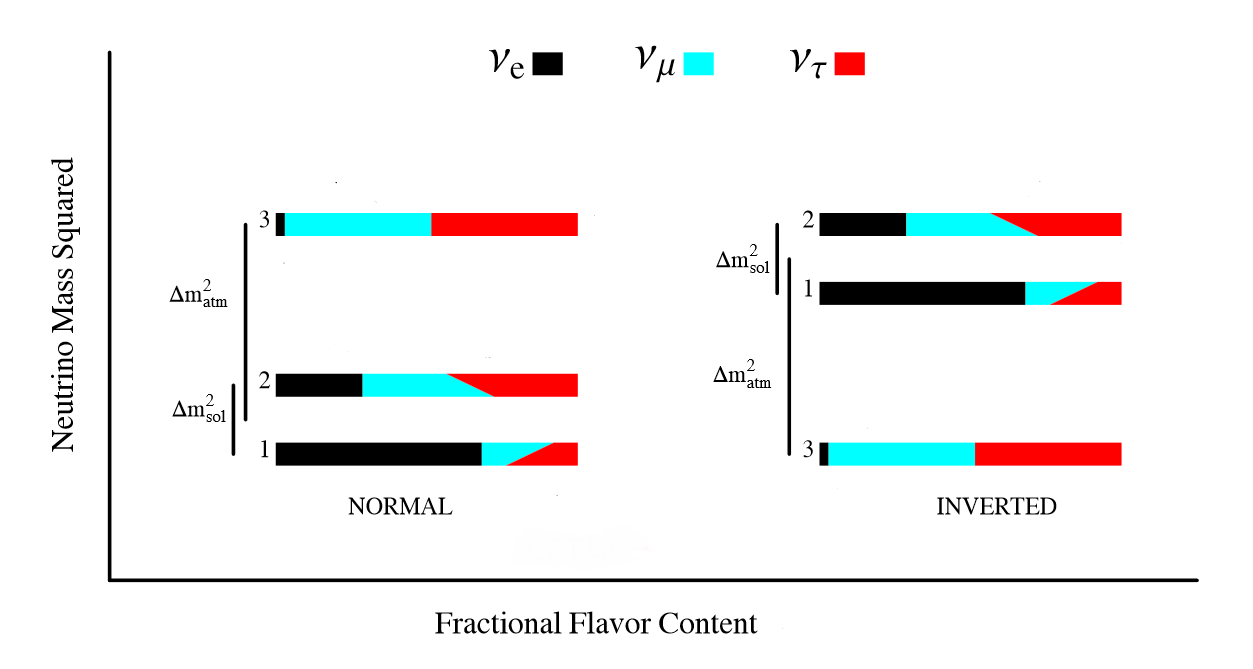
\includegraphics[scale=0.4]{neutrinos.png}
\captionof{figure}{The two hierarchies of neutrino mass states.  Black, teal, and red indicated the three flavors of neutrinos, while one, two, and three indicated the three mass states~\cite{Parke}.}
\label{neutrinos}
\end{center}


The density parameter of neutrinos is given by
\[\Omega_\nu=\frac{\rho_\nu}{\rho_c}=\frac{1}{h^2}\sum_{i=1}^3 \frac{g_i m_i}{90~\text{eV}}\]
where $g_i = 1$ for Majorana neutrinos (own antiparticle) and $g_i = 2$ for Dirac neutrinos (distinct antiparticles)~\cite{Pastor}. Using the lower mass limit of the neutrino and assuming Majorana neutrinos, this suggests a lower limit on the neutrino density parameter of $\Omega_\nu \gtrsim 0.00122$.  Thus, neutrinos do provide some contribution to the nonbaryonic dark matter density parameter.  

To find an upper limit on the neutrino contribution to the nonbaryonic dark matter density parameter is is necessary to distinguish hot dark matter from cold dark matter.  Hot dark matter is composed of particles that have zero or nearly-zero mass.  Special relativity requires that the massless particles move at the speed of light, and that the nearly-massless particles move close to the speed of light if they have any substantial momentum.  As a result hot dark matter forms very hot gases.  Cold dark matter is composed of particles that at sub-relativistic velocities.  With their low masses neutrinos fall under the hot dark matter category.  A combination of galaxy clustering measurements, CMB observations, and Lyman-$\alpha$ observations give an upper limit on the hot dark matter contribution of $\Omega_\nu \lesssim 0.0155$, thus neutrinos and other hot dark matter particles cannot be the primary contribution to the nonbaryonic dark matter density parameter~\cite{Spergel}.

\subsubsection{WIMPs and SUSY} \label{WIMPSandSUSY}

If we assume cold dark matter (CDM) particles were in thermal equilibrium with the other standard model particles during the early stages ($<$1 ns) of the universe, it is possible to calculate the CDM density parameter.  As the temperature, $T$, of the universe cools, the particles with masses $m > T$ will diminish exponentially.  Once the temperature of the universe cooled below the CDM mass scale the creation of these particles would have ceased.  At this time the CDM particles which still existed would have continued annihilating with one another.  As time went on, CDM annihilation became less and less likely due to their dwindling abundance.  Once the expansion rate of the universe, given by Hubble's constant, exceeded the CDM annihilation rate, the CDM particles dropped out of thermal equilibrium and the CDM density became fixed.  

The density parameter for CDM is approximately given by
\[\Omega_{CDM} h^2 \simeq \frac{T_0^3}{M_{Pl} \langle \sigma_A \nu \rangle} \]
where $\sigma_A$ is the total annihilation cross section of CDM particles, $\nu$ is the relative velocity of CDM particles, $T_0$ is the equilibrium temperature at freeze out, $M_{Pl}$ is the Planck mass, $c$ is the speed of light, and $\langle ... \rangle$ represents an average over the thermal distribution of CDM particle velocities~\cite{Kolb,Jungman}. Remarkably, for the total density parameter of the universe to equal unity, as required by cosmological observations, an annihilation cross section on the order of particles interacting on the electroweak scale ($\sim 10^{-9}$~GeV$^{-2}$) is required for CDM particles. This result is the main motivation behind suspecting weakly interacting massive particles (WIMPs) as the dominant contribution to the nonbaryonic dark matter density parameter.  

Supersymmetry (SUSY) is a symmetry of space-time which has been proposed in an effort to unify the electroweak, strong, and gravitational forces.  This theory offers some insight into the nature of WIMPs.  SUSY requires that a super-symmetric partner particle exists for each particle in the standard model.  These partners go by the names of sleptons (partners of leptons), squarks (partners of quarks), gauginos (partners of gauge bosons), and higgsinos (partners of Higgs bosons).  Sleptons and squarks have spin zero, while gauginos and higgsinos have spin one-half.  Since none of these super-symmetric particles have been discovered it is thought they are far more massive than their standard model counterparts, and thus that super-symmetry is not an explicit symmetry of nature.
  
Goldberg~\cite{Goldberg} and Ellis~\cite{Ellis} have suggested that neutral gauginos and neutral higgsinos can mix together in a superposition known as the neutralino, $\chi$.  In most SUSY models, the neutralino is the lightest super-symmetric particle (LSP).  In models which conserve R-parity (a new quantum number distinguishing SUSY particles from standard model particles) the LSP is stable, making it a prime candidate particle for dark matter.  The expected cross section of neutralinos interacting via inelastic collisions with nucleons is dependent on the allowed regions of parameter space in the SUSY model being used.  
%Results from the WMAP satellite refined this parameter space, concluding that the density parameter of neutralinos would be  $0.192 < \Omega_\chi < 0.263$~\cite{Spergel,Bennett,Arnowitt}.

The neutralino is one of many candidate particles suggested for WIMPs, and as previously mentioned, WIMPs are not the only candidate for dark matter.  In the following sections we will briefly discuss some of the other candidates before returning to the discussion of WIMPs in Chapter~\ref{Chapter2}.

\subsubsection{Axions and Axinos}
Quantum chromodynamics (QCD) is a theory describing the strong interaction between quarks and gluons, which make up hadrons.  In particle physics there exists a proposed symmetry of nature referred to as charge conjugation parity symmetry (CP-Symmetry).  CP-Symmetry postulates that particles should behave the same if they are replace by their own antiparticle (C symmetry), and then have their parity reversed (P symmetry). Within QCD there is no theoretical reason to assume CP-symmetry exists.  However, when a CP-violation term is included in the QCD lagrangian its coefficient has been experimentally determined to be less than $10^{-10}$~\cite{Baluni}. This unexpected result is known as the strong CP problem in quantum chromodynamics.    To reconcile this, a new symmetry known as the Peccei-Quinn theory has been proposed.  This theory postulates the existence of a new pseudoscalar particle called the axion.  According to the Peccei-Quinn theory, axions would be electrically neutral, stable, low mass ( $1\mu$~eV - $1$~eV) particles that have very low interaction cross sections for the strong and weak forces. Therefore, axions satisfy all of the requirements to be a dark matter candidate.  

If axions exists, they would be observable through an $a \rightarrow \gamma \gamma$ interaction.  Figure~\ref{AxionSearch} shows limits that various axion detection experiments have placed on the effective coupling of this process. Dark matter axions would lie somewhere between the lines labeled as "KSVZ" and "DFSZ". (KSVZ and DFSZ are acronyms for two "invisible axion" theories which describe the axion as a dark matter candidate) At the top of Figure~\ref{AxionSearch}, axions would be observable through seismic signatures in the Sun, as well as through scattering processes in germanium crystals.  These processes have not been observed, so they are used to exclude possible values of the coupling constant.  In the upper right, the optical photons from axion decay in the halos around astrophysical object would be observable in telescopes. Axion emission from astrophysical objects would affect the evolution of those objects, placing an upper limit on the coupling constant at $\sim 10^{-10}$ GeV$^{-1}$.  Axion emissions in supernovae would shorten the duration of neutrino bursts detected on Earth seen from SN 1987a.  These observations place the strongest upper limit on the coupling constant at $\sim 10^{-13}$ GeV$^{-1}$. (Not depicted in the figure)  These limits produce a small window between 1-100 $\mu$eV in which axion dark-matter can exist, which the Axion Dark Matter Experiment (ADMX) experiment is currently searching~\cite{AxionReview}.

\begin{center}
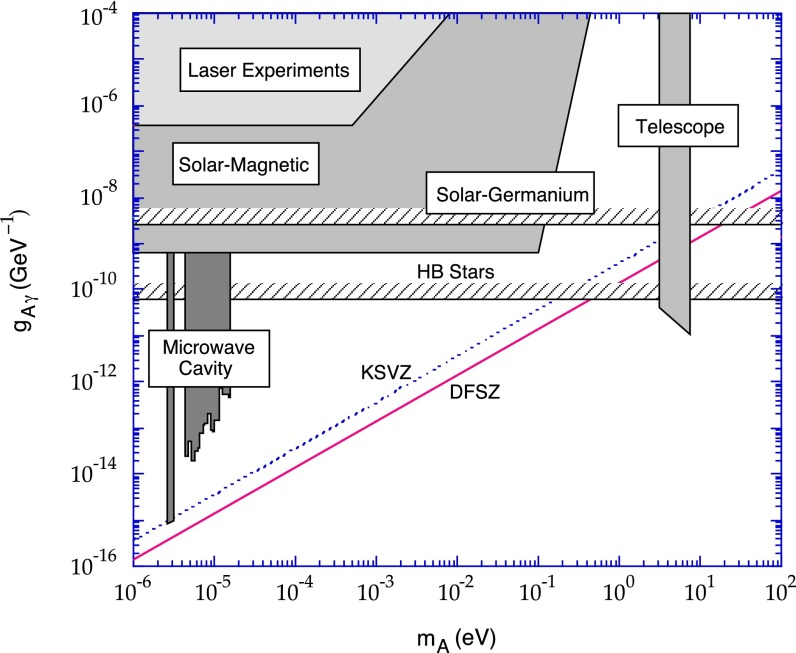
\includegraphics[scale=3]{AxionSearch.jpg}
\captionof{figure}{Historical limits placed on axion masses and photon coupling constants.  If dark matter axions exist, they would lie between the lines labeled KSVZ and DFSZ~\cite{AxionReview}.}
\label{AxionSearch}
\end{center}


%Axions would have been gravitationally slowed in the early universe, causing them to behave like cold dark matter despite their low mass.

%The axino arises when SUSY is introduced to the Peccei-Quinn theory, resulting in a supersymmetric partner to the axion known as the axino.

\subsubsection{Gravitons and Gravitinos}
In quantum field theory, the graviton is a hypothetical  elementary particle which mediates the gravitational force.  As with axions and axinos, when SUSY is introduced to quantum field theory a super-symmetric partner to the graviton is predicted to exist, known as the gravitino.  In some models, gravitinos are the LSP in SUSY and are thus a candidate particle for dark matter.

\subsubsection{WIMPzillas}
WIMPzillas are supermassive dark matter particles which arise when one considers the possibility that dark matter might be composed of nonthermal supermassive states. These particles would have a mass many orders of magnitude higher than the weak scale~\cite{Chung}. Studies have shown that for stable particles with masses close to $10^{13}$~GeV  WIMPzillas would be produced in sufficient abundance to give $\Omega \approx 1$ for the total density parameter of the universe.  

It should be noted that the discussion of this section does not encompass all of the alternatives to WIMPs.   Although these other dark matter candidates offer intriguing explanations to the dark matter problem, the next chapter will focus on the experimental detection of WIMPs.

%http://arxiv.org/pdf/hep-ph/0404175v2.pdf was used as a heavy resource here.. not sure where to cite it though

\subsection{Outline of the Thesis}

In this chapter, we discussed the evidence for the existence of dark matter, and the popular WIMP conjecture.  In the next chapter, we will provide an overview of many experiments searching for WIMPs, before describing one such experiment, the LUX detector, in Chapter~\ref{LUXChap}. The remaining chapters will be used to discuss original work related to LUX. 

In Chapter~\ref{TritiumChapter} we describe a novel tritiated methane calibration source that was used to measure LUX's electron recoil response with unprecedented precision.  A detailed description of the R\&D efforts that led to the successful deployment of the source is included, and the results from the first calibration data set are discussed.


 In Chapter~\ref{StandardCalibrations}, we discuss the position dependent signal corrections used in LUX's Run3 data analysis.  These corrections depend on a $^{83m}$Kr calibration source, and remove any position dependence in the detector's gain factors. Alternative methods for producing signal corrections are also presented.
 
 In Chapter~\ref{CombinedEnergyModel}, we discuss a number of energy scale calibrations that were used in the LUX detector.  These methods use multiple mono-energetic sources and the tritiated methane beta spectrum to determine the (now position independent) gain factors for the detector's signals.  
 
 In Chapter~\ref{Run04Corrections}, we discuss the position dependent signal corrections used in LUX's Run4 data analysis.  LUX's Run4 data was complicated by a non-uniform drift field, and a number of novel techniques were developed to recover the quality of data that was collected in Run3.  These techniques draw from the calibration sources and analysis methods that are discussed in each of the previous chapters.